\section{Vehicle-Side Planning and Anti-Rollover Control}

\subsection{Vehicle-Side Emergency Trajectory Replanning}

The vehicle-side planner is a local safety fallback rather than an independent replacement for cloud-side predictive planning. It is activated when the cloud trajectory conflicts with local perception, a sudden obstacle appears, the rollover margin decreases below a preset threshold, or a cloud message is delayed or inconsistent. The planner uses the cloud trajectory $\tau_c$ as an initial solution and reconstructs a short-horizon trajectory that satisfies local collision, road-boundary, actuator, and rollover constraints.

The planner uses a simplified articulated tanker model for fast prediction. Following the defense-oriented design, the tractor is represented by a kinematic model because it is directly controlled, whereas the trailer keeps speed-dependent amplification and rollover-response terms to preserve high-speed tracking and stability effects. The kinematic part describes the tractor rear-axle position $(X_{1r},Y_{1r})$, tractor heading $\psi_1$, and trailer heading $\psi_2$:
\begin{equation}
\begin{cases}
\dot{X}_{1r}=v_{1x}\cos\psi_1,\\
\dot{Y}_{1r}=v_{1x}\sin\psi_1,\\
\dot{\psi}_1=\frac{v_{1x}}{L_1}\tan\delta,\\
\dot{\psi}_2=K_v\frac{v_{1x}}{L_2}
\left(\frac{L_h}{L_1}\tan\delta\cos\gamma_g+\sin\gamma_g\right),
\end{cases}
\label{eq:vehicle_planning_model}
\end{equation}
where $\gamma_g=\psi_1-\psi_2$ is the articulation angle and $K_v$ is a speed-dependent trailer amplification factor that approximates high-speed tire-slip effects. A low-order linear rollover model is appended to predict LTR under candidate trajectories.

To reduce the number of interaction cases, local multimodal predictions of surrounding vehicles are screened against the cloud reference. For each predicted surrounding-vehicle trajectory $\tau_i^j$, the planner constructs its swept occupancy $\sigma_{\tau_i^j}$ and checks its earliest intersection with the swept occupancy of $\tau_c$. The vehicle whose trajectory first intersects the cloud reference is selected as the key vehicle. The planner then builds two representative scenarios: the most probable scenario $S_\alpha$ and the most dangerous scenario $S_\beta$ that includes the key vehicle's conflicting mode above a probability threshold.

\begin{figure}[t]
  \centering
  \subfloat[Key vehicle selection\label{fig:key_vehicle_selection}]
    {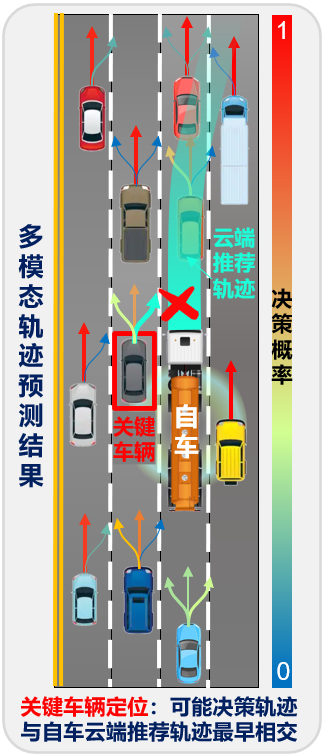
\includegraphics[width=0.31\linewidth]{fig/chap3/scenario_selection1.png}}
  \subfloat[Dual-scenario construction\label{fig:dual_scenario_construction}]
    {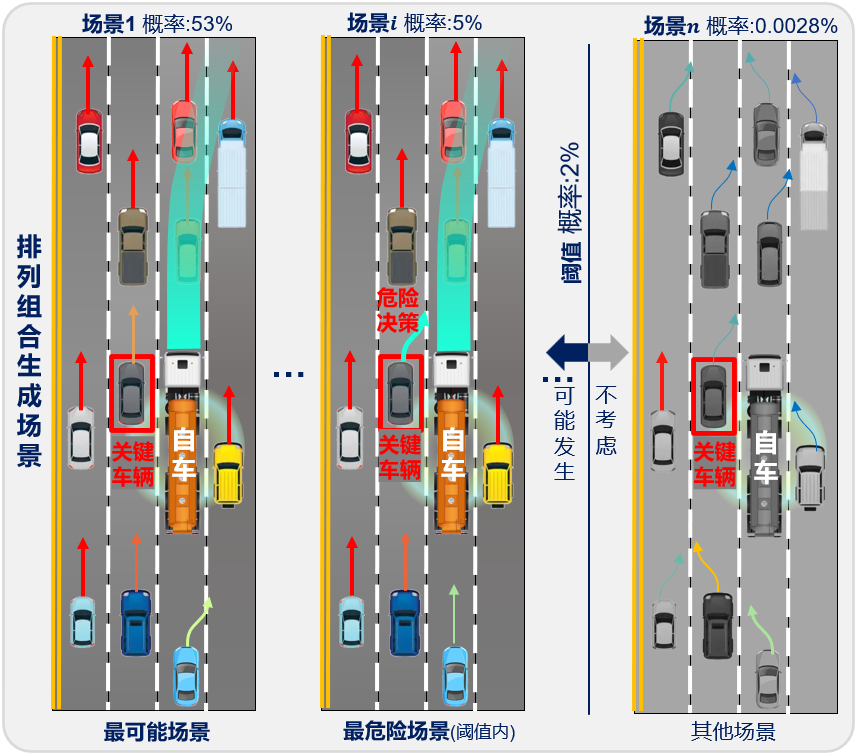
\includegraphics[width=0.63\linewidth]{fig/chap3/scenario_selection2.png}}
  \caption{Vehicle-side emergency scenario screening based on the cloud reference trajectory.}
  \label{fig:vehicle_emergency_scenarios}
\end{figure}

The emergency trajectory is solved with constrained iterative LQR (CILQR). A nominal optimal-control problem is
\begin{equation}
\begin{aligned}
\min_{u_{0:N_p-1}}\quad
& \ell_f(x_{N_p})+\sum_{k=0}^{N_p-1}\ell(x_k,u_k)\\
\mathrm{s.t.}\quad
&x_{k+1}=f_v(x_k,u_k),\quad x_0=x_{start}.
\end{aligned}
\label{eq:cilqr_nominal}
\end{equation}
Obstacle avoidance, road boundaries, steering limits, articulation limits, and rollover limits are introduced through control barrier penalties. For a constraint $c_k(x_k)\leq0$, the penalty is
\begin{equation}
  b_k=q_1\exp(q_2 c_k(x_k)).
  \label{eq:cbf_penalty}
\end{equation}
The rollover constraint is tightened along the prediction horizon to compensate for simplified-model uncertainty:
\begin{equation}
  \mathcal{L}_{lim}(t)=\mathcal{L}_{lim}^{0}\exp(-t/\tau_{decay}).
  \label{eq:ltr_tightened}
\end{equation}
The two scenario trajectories share an initial segment, so the vehicle can preserve performance in $S_\alpha$ while remaining feasible if $S_\beta$ occurs. In implementation, an outer loop adjusts a danger factor according to constraint violation in $S_\beta$, while an inner CILQR loop optimizes the shared-prefix trajectory and the two branches. When the local evidence confirms the dangerous mode, the vehicle switches to the already feasible emergency branch. This contingency structure is the vehicle-side degraded-safety mechanism when the cloud reference no longer provides a sufficient safety margin.

\subsection{Coupled Tank-Truck Dynamics for Control}

The high-frequency controller uses a more detailed control-oriented model than the emergency planner. The model couples a semi-trailer vehicle model with an equivalent liquid-sloshing model. The vehicle part contains tractor lateral, yaw, and roll dynamics, trailer yaw and roll dynamics, longitudinal speed dynamics, and global pose. The liquid part is represented by a linearized double-pendulum (LDP) model whose parameters can be updated from a higher-fidelity sliding telescopic libra (STL) sloshing model. The STL model is introduced to capture longitudinal-lateral coupled sloshing, chamber-to-chamber liquid transfer, and yaw/roll excitation effects that are difficult to express with a conventional two-dimensional pendulum. The STL model is used for high-fidelity rapid simulation and offline or periodic re-linearization; the LDP model is used inside the MPC to preserve real-time solvability.

\begin{figure}[t]
  \centering
  \subfloat[Coordinate definition\label{fig:coord_def_journal}]
    {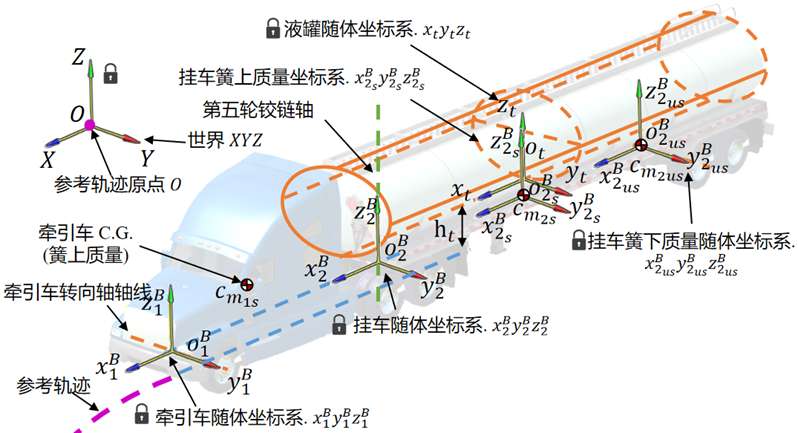
\includegraphics[width=0.64\linewidth]{fig/chap4/coord_def.png}}
  \subfloat[Roll-plane simplification\label{fig:roll_plane_model_journal}]
    {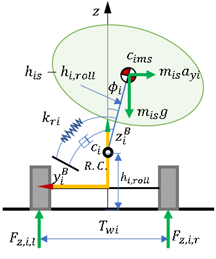
\includegraphics[width=0.28\linewidth]{fig/chap4/trailer_model_lat.png}}\\
  \subfloat[Yaw-plane simplification\label{fig:yaw_plane_model_journal}]
    {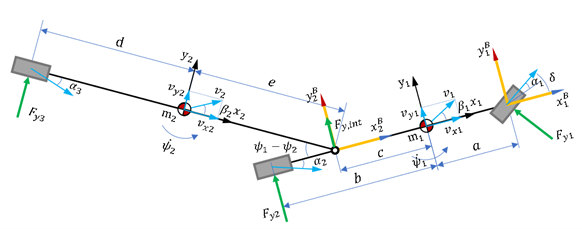
\includegraphics[width=0.95\linewidth]{fig/chap4/trailer_model_lon.png}}
  \caption{Control-oriented coupled semi-trailer tanker-truck model.}
  \label{fig:coupled_vehicle_model}
\end{figure}

The control-oriented state vector is
\begin{equation}
\begin{aligned}
x=&[v_{1y},\dot{\psi}_1,\phi_1,\dot{\phi}_1,
v_{2y},\dot{\psi}_2,\phi_2,\dot{\phi}_2,\\
&\theta_1,\dot{\theta}_1,\theta_2,\dot{\theta}_2,
v_{1x},\psi_1,Y_1,X_1]^T,
\end{aligned}
\label{eq:control_state}
\end{equation}
where the subscripts 1 and 2 denote tractor and trailer, respectively, and $\theta_1,\theta_2$ are the equivalent sloshing angles. The controller input is
\begin{equation}
u=[\delta,\ p_{brk}^{L1},\ p_{brk}^{R1},\ p_{brk}^{L2},\ p_{brk}^{R2},\ v_{des}]^T.
\label{eq:control_input}
\end{equation}
The differential braking variables are grouped by left/right and tractor/trailer axle groups. This input structure allows the controller to coordinate active steering, differential braking, and desired speed.

The continuous-time linearized model at each control step is
\begin{equation}
  \dot{x}=A_c x+B_c u,
  \label{eq:continuous_ltv}
\end{equation}
where $A_c$ and $B_c$ are updated using the current longitudinal speed, roll state, articulation state, and liquid-equivalent parameters. With zero-order hold, the discrete-time model is
\begin{equation}
  x_{k+1}=A_d x_k+B_d u_k.
  \label{eq:discrete_control_model}
\end{equation}
The STL model used for high-fidelity sloshing approximation contains longitudinal-lateral coupled liquid-mass transfer and additional forces/moments. The source thesis reports that an identified STL model predicts 15 s of liquid-force response in about 5 ms in MATLAB and less than 1 ms after C++ compilation, while maintaining the same force/moment trends as CFD over the tested orthogonal excitation cases. For online MPC, a residual reinforcement-learning re-linearization module maps STL states to LDP parameter and state corrections, so the LDP model preserves the dominant sloshing response over the prediction horizon.

\subsection{Multi-Constraint Anti-Rollover MPC}

The MPC is the final safety layer of the proposed vehicle-cloud system. It solves an incremental linear MPC problem to track the selected reference trajectory while suppressing sloshing and preventing rollover. Unlike a pure path-tracking controller, it is expected to reject an unsafe reference by introducing controlled path deviation, speed reduction, and differential braking when the rollover margin becomes small. The output vector is
\begin{equation}
  y=[Y_1,\ X_1,\ \psi_1,\ \dot{\theta}_1,\ \dot{\theta}_2,\ \mathrm{LTR}_{eql},\ v_{1x}]^T.
  \label{eq:mpc_output}
\end{equation}
Absolute position $(Y_1,X_1)$ is used rather than only lateral error, because it better preserves high-order vehicle-liquid dynamics over the 2--3 s control prediction horizon.

For incremental MPC, define
\begin{equation}
  \xi_k=\begin{bmatrix}x_k\\u_{k-1}\end{bmatrix},\quad
  \xi_{k+1}=A\xi_k+B\Delta u_k,\quad
  \eta_k=C\xi_k.
  \label{eq:incremental_mpc_state}
\end{equation}
Stacking the predicted outputs over horizon $N_p$ yields
\begin{equation}
  Y=\Psi\xi_k+\Theta\Delta U,
  \label{eq:stacked_output}
\end{equation}
where $\Delta U=[\Delta u_k^T,\ldots,\Delta u_{k+N_c-1}^T]^T$. The quadratic cost is
\begin{equation}
\begin{aligned}
J=&(Y-Y_r)^TQ_Q(Y-Y_r)+\Delta U^TR_R\Delta U+\rho\epsilon^2\\
=&\frac{1}{2}
\begin{bmatrix}\Delta U\\\epsilon\end{bmatrix}^T
\begin{bmatrix}H&0\\0&\rho\end{bmatrix}
\begin{bmatrix}\Delta U\\\epsilon\end{bmatrix}
+\begin{bmatrix}g\\0\end{bmatrix}^T
\begin{bmatrix}\Delta U\\\epsilon\end{bmatrix}
 + Const.
\end{aligned}
\label{eq:mpc_cost}
\end{equation}
The reference $Y_r$ contains path points, desired heading, desired speed, zero sloshing-rate reference, and a safe rollover-index reference.

The constraints include actuator bounds,
\begin{equation}
  U_{min}\leq U_t+A_t\Delta U\leq U_{max},
  \label{eq:mpc_input_bound}
\end{equation}
input-increment bounds,
\begin{equation}
  \Delta U_{min}\leq\Delta U\leq\Delta U_{max},
  \label{eq:mpc_delta_bound}
\end{equation}
soft output constraints,
\begin{equation}
\begin{cases}
\Pi\Theta\Delta U-\epsilon\leq\Pi(Y_{max}-E),\\
-\Pi\Theta\Delta U-\epsilon\leq\Pi(Y_{min}-E),
\end{cases}
\label{eq:mpc_output_constraint}
\end{equation}
and slack bounds $\epsilon_{min}\leq\epsilon\leq\epsilon_{max}$. Here, $E=\Psi\xi_k$, and $\Pi$ is a constraint-compression mapping. The most important output constraint is
\begin{equation}
  |\mathrm{LTR}_{eql}|\leq \mathrm{LTR}_{max}+\epsilon,
  \label{eq:mpc_ltr_constraint}
\end{equation}
where $\mathrm{LTR}_{max}=0.75$ is used in the simulations and scaled experiments. Sloshing suppression is handled by penalizing and constraining $\dot{\theta}_1$ and $\dot{\theta}_2$, and speed constraints prevent unrealistic compensation between braking and desired-speed commands.

\begin{figure}[t]
  \centering
  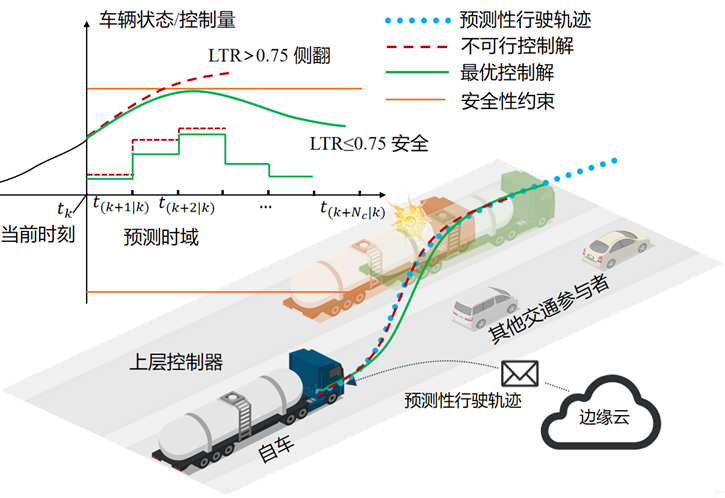
\includegraphics[width=0.78\linewidth]{fig/chap4/mpc_illust.png}
  \caption{Multi-constraint MPC for tracking, sloshing suppression, and rollover prevention.}
  \label{fig:mpc_scheme_journal}
\end{figure}

The resulting QP is solved by qpOASES. To reduce the peak solution time for the high-dimensional state and input space, a moving-block decision compression and constraint-set compression are used. The source thesis reports that this compression has less than 1\% influence on control optimality for the tested setting while reducing peak QP solution time. This acceleration is important because the control layer is the final onboard safety barrier and cannot rely on cloud-side replanning during fast roll and sloshing transients.

\subsection{Real-Time Implementation}

The vehicle-side implementation uses a hierarchical execution logic. At each vehicle-planning cycle, the local planner checks the cloud reference against local perception and predicted rollover margins. If the reference remains safe, the controller tracks $\tau_c$. Otherwise, CILQR generates a local emergency trajectory $\tau_v$, and the controller tracks $\tau_v$. At each control cycle, the state estimator updates vehicle pose, roll states, yaw states, speed, and equivalent liquid states. The LTV model is re-linearized, the MPC QP is solved, and only the first input is applied.

The scaled-vehicle implementation runs the controller at 20 Hz. The source thesis reports an average MPC solution time of 15.4 ms and a peak solution time below 25 ms in model-truck experiments. The controller can therefore serve as the final high-frequency safety layer under the tested experimental conditions.
